\documentclass{article}
\usepackage{listings}
\usepackage{color}
\usepackage{fancyhdr}
\usepackage{extramarks}
\usepackage{amsmath}
\usepackage{amsthm}
\usepackage{amsfonts}
\usepackage{tikz}
\usepackage{bold-extra}
\usepackage[plain]{algorithm}
\usepackage{algpseudocode}
\usepackage{pdfpages}
\usepackage[
    backend=biber,
    style=gb7714-2015,
    gbalign=gb7714-2015,
    gbnamefmt=lowercase,
    gbpub=false,
    doi=false,
    url=false,
    eprint=false,
    isbn=false,
]{biblatex}
\addbibresource{misc/ref.bib}
\usetikzlibrary{automata,positioning}

\definecolor{mygreen}{RGB}{28,172,0} % color values Red, Green, Blue
\definecolor{mylilas}{RGB}{170,55,241}
\definecolor{backcolour}{rgb}{0.95,0.95,0.92}
%
% Basic Document Settings
%

\topmargin=-0.45in
\evensidemargin=0in
\oddsidemargin=0in
\textwidth=6.5in
\textheight=9.0in
\headsep=0.25in

\linespread{1.1}

\pagestyle{fancy}
\lhead{\hmwkAuthorName}
\rhead{\leftmark}
\lfoot{\lastxmark}
\cfoot{\thepage}

\renewcommand\headrulewidth{0.4pt}
\renewcommand\footrulewidth{0.4pt}

\setlength\parindent{0pt}

\setcounter{secnumdepth}{0}

\newcommand{\hmwkTitle}{Homework\ \#4}
\newcommand{\hmwkClass}{24352}
\newcommand{\hmwkAuthorName}{\textbf{Daniel Deng}}

%
% Title Page
%

\title{
    \vspace{2in}
    \textmd{\textbf{\hmwkClass:\ \hmwkTitle}}\\
    \vspace{3in}
}

\author{\hmwkAuthorName}
\date\today

\renewcommand{\part}[1]{\textbf{\large Part \Alph{partCounter}}\stepcounter{partCounter}\\}

%
% Various Helper Commands
%

% Useful for algorithms
\newcommand{\alg}[1]{\textsc{\bfseries \footnotesize #1}}

% For derivatives
\newcommand{\deriv}[1]{\frac{\mathrm{d}}{\mathrm{d}x} (#1)}

% For partial derivatives
\newcommand{\pderiv}[2]{\frac{\partial}{\partial #1} (#2)}

% Integral dx
\newcommand{\dx}{\mathrm{d}x}

% Alias for the Solution section header
\newcommand{\solution}{\textbf{\large Solution}}

% Probability commands: Expectation, Variance, Covariance, Bias
\newcommand{\E}{\mathrm{E}}
\newcommand{\Var}{\mathrm{Var}}
\newcommand{\Cov}{\mathrm{Cov}}
\newcommand{\Bias}{\mathrm{Bias}}

\begin{document}

%% matlab code
\lstset{language=Matlab,%
    %basicstyle=\color{red},
    backgroundcolor = \color{backcolour},
    breaklines=true,%
    morekeywords={matlab2tikz},
    keywordstyle=\color{blue},%
    morekeywords=[2]{1}, keywordstyle=[2]{\color{black}},
    identifierstyle=\color{black},%
    stringstyle=\color{mylilas},
    commentstyle=\color{mygreen},%
    showstringspaces=false,%without this there will be a symbol in the places where there is a space
    numbers=left,%
    numberstyle={\tiny \color{black}},% size of the numbers
    numbersep=9pt, % this defines how far the numbers are from the text
    emph=[1]{for,end,break},emphstyle=[1]\color{red}, %some words to emphasise
    %emph=[2]{word1,word2}, emphstyle=[2]{style},    
}


\maketitle

\pagebreak

\section{Problem 1}
    State space representation from differential equations.

    \subsection{a)} 
    $2\ddot{x} + 4\dot{x} + 4x=3u$, where the state vector is 
    $\begin{bmatrix}
        x \\
        \dot{x}
    \end{bmatrix}$.
    The out put is x.
    \subsubsection{\textit{ Sol. }}
    $\ddot{x} + 2\dot{x} + 2x=1.5u$ $\Rightarrow$ 
    $\left\{
        \begin{array}{lr}
        \dot{x} = 0x + \dot{x} \\
        \ddot{x} = -2x -2\dot{x} + 1.5u
        \end{array}
    \right.$, thus

    \begin{align}
        \dot{\textbf{x}} &=
        \begin{bmatrix}
            \dot{x} \\
            \ddot{x}
        \end{bmatrix} = 
        \begin{bmatrix}
            0 & 1 \\
            -2 & -2
        \end{bmatrix}
        \begin{bmatrix}
            x \\
            \dot{x}
        \end{bmatrix} + 
        \begin{bmatrix}
            0\\
            1.5
        \end{bmatrix}
        u
        \\
        y&=
        \begin{bmatrix}
            x
        \end{bmatrix} =
        \begin{bmatrix}
            1 & 0
        \end{bmatrix}
        \begin{bmatrix}
            x \\
            \dot{x}
        \end{bmatrix} + 
        \begin{bmatrix}
            0
        \end{bmatrix}
        u
    \end{align}

    We get:

    \begin{equation}
        \textbf{A} =
        \begin{bmatrix}
            0 & 1 \\
            -2 & -2
        \end{bmatrix}, 
        \textbf{B} =
        \begin{bmatrix}
            0\\
            1.5
        \end{bmatrix}, 
        \textbf{C} =
        \begin{bmatrix}
            1 & 0
        \end{bmatrix}, 
        \textbf{D} =
        \begin{bmatrix}
            0
        \end{bmatrix}
    \end{equation}

    \subsection{b)} 
    $2\ddot{x} + 4\dot{x} + 4x=3u$, where the state vector is 
    $\begin{bmatrix}
        x + \dot{x} \\
        \dot{x}
    \end{bmatrix}$.
    The out put is x.

    \subsubsection{\textit{ Sol. }}
    $\left\{
        \begin{array}{lr}
        \dot{x} + \ddot{x} = \dot{x} + (-2x -2\dot{x} + 1.5u) = -2(x + \dot{x}) + \dot{x} + 1.5u\\
        \ddot{x} = -2x -2\dot{x} + 1.5u = -2(x + \dot{x}) + 0\dot{x} + 1.5u \\
        x = (x + \dot{x}) + (-1)\dot{x}
        \end{array}
    \right.$, thus

    \begin{align}
        \dot{\textbf{x}} &=
        \begin{bmatrix}
            \dot{x} + \ddot{x}\\
            \ddot{x}
        \end{bmatrix} = 
        \begin{bmatrix}
            -2 & 1 \\
            -2 & 0
        \end{bmatrix}
        \begin{bmatrix}
            x + \dot{x}\\
            \dot{x}
        \end{bmatrix} + 
        \begin{bmatrix}
            1.5\\
            1.5
        \end{bmatrix}
        u
        \\
        y&=
        \begin{bmatrix}
            x
        \end{bmatrix} =
        \begin{bmatrix}
            1 & -1
        \end{bmatrix}
        \begin{bmatrix}
            x + \dot{x}\\
            \dot{x}
        \end{bmatrix} + 
        \begin{bmatrix}
            0
        \end{bmatrix}
        u
    \end{align}

    We get:

    \begin{equation}
        \textbf{A} =
        \begin{bmatrix}
            -2 & 1 \\
            -2 & 0
        \end{bmatrix}, 
        \textbf{B} =
        \begin{bmatrix}
            1.5\\
            1.5
        \end{bmatrix}, 
        \textbf{C} =
        \begin{bmatrix}
            1 & -1
        \end{bmatrix}, 
        \textbf{D} =
        \begin{bmatrix}
            0
        \end{bmatrix}
    \end{equation}
    

    \subsection{c)}
    Using the A,B,C,D matrices found in parts (a) and (b), use Matlab's step command to simulate the step responses to both systems. How do these step responses compare and does that comparison make sense? 
    \subsubsection{\textit{ Sol. }}
    Matlab code:
    \lstinputlisting{codes/Question1c.m}
    Result:
    \begin{figure}[htp]
        \centering
        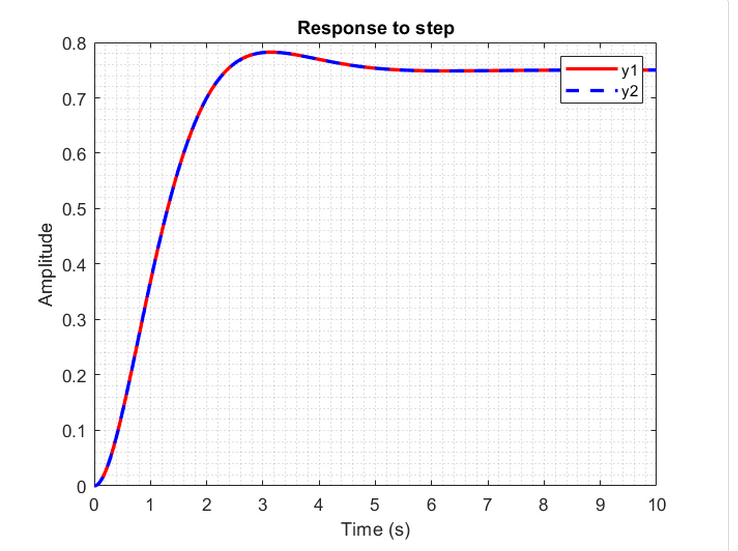
\includegraphics[width=15cm]{images/Q1_c_fig.png}
        \caption{Step Response}
        \label{fig:Q1c}
    \end{figure}

    We can tell from Fig.\ref{fig:Q1c} that the step responses are exactly the same.
    This make sense because we are representing the same system, and the output is the same for the two representations. 

\pagebreak
\section{Problem 2}
State space representation of a 2-mass system.

For the following mechanical system, there is one input, $f$, and two outputs: the position of the first mass, $z_1$, and the distance between the masses, $z_1 - z_2$.

\begin{figure}[htp]
    \centering
    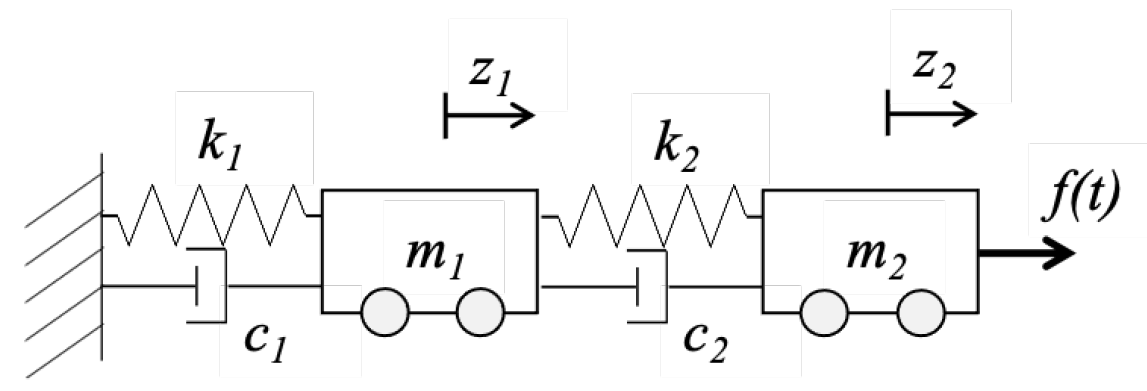
\includegraphics[width=15cm]{images/Q2.png}
\end{figure}

\subsection{a)}
Write the state equation, $\dot{x}=Ax+Bu$, where $x$ is a state vector that you choose, $A$ is the system matrix, $B$ is the input matrix, and $u$ is the input.
\subsubsection{\textit{ Sol. }}

First we identify all energy storage elements:

\begin{table}[ht]
    \centering
    \begin{tabular}{c | c}
        Energy Storage Elements & State variable
        \\
        \hline
        $m_1$ (Kinetic) & $\dot{z_1}$ \\
        $m_2$ (Kinetic) & $\dot{z_2}$ \\
        $k_1$ (Potential) & $z_1$ \\
        $k_2$ (Potential) & $z_2 - z_1$
    \end{tabular}
\end{table}

From all energy storage elements we define the state vector: $\textbf{x} = 
\begin{bmatrix}
    x_1\\
    x_2\\ 
    x_3\\ 
    x_4
\end{bmatrix} = 
\begin{bmatrix}
    z_1\\
    z_2 - z_1\\ 
    \dot{z_1}\\ 
    \dot{z_2}
\end{bmatrix}$, and input $u = f$

Draw FBD to analyze system dynamics: 
\begin{figure}[htp]
    \centering
    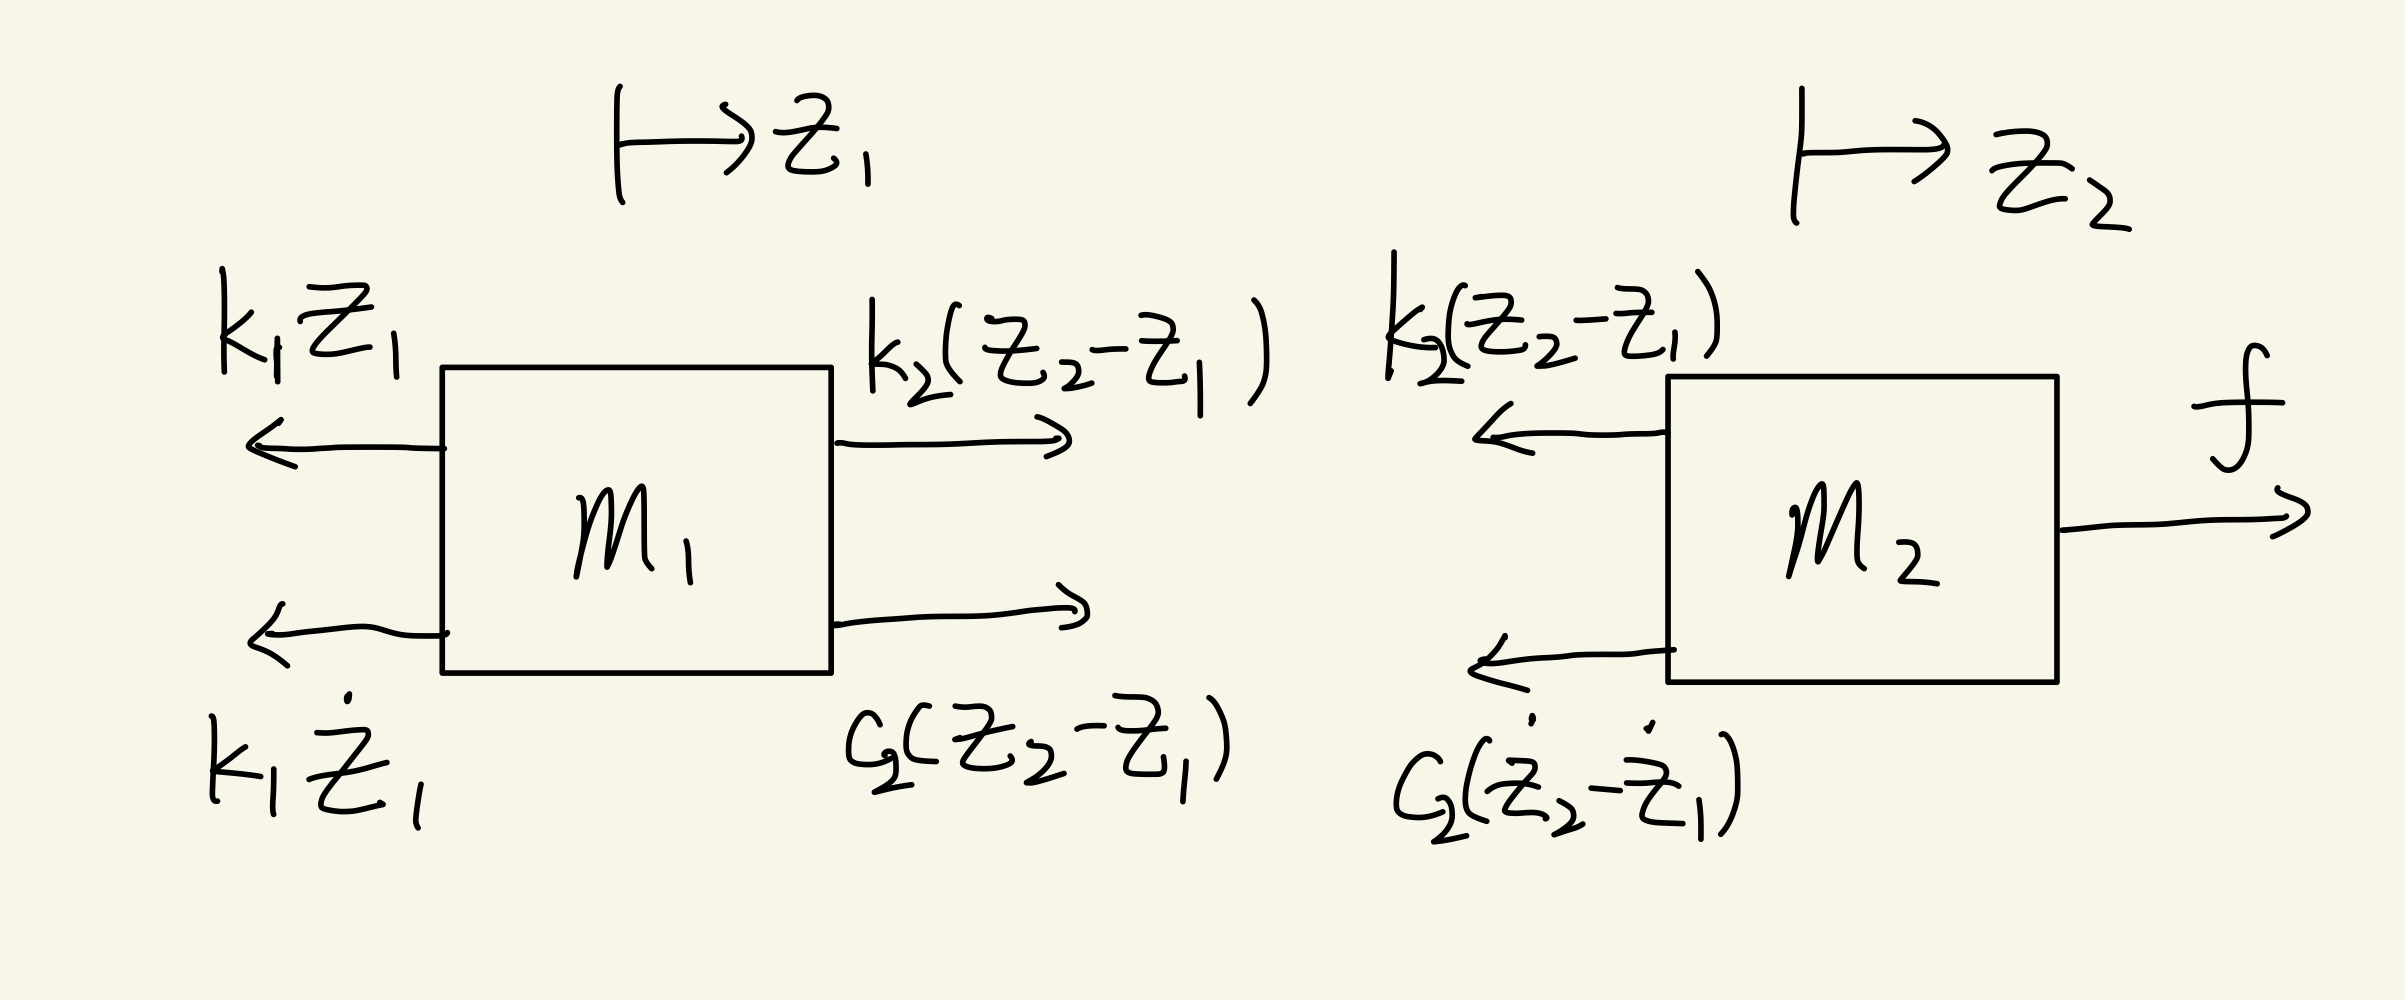
\includegraphics[width=10cm]{images/Q2_FBD.png}
    \caption{Free body diagram}
    \label{fig:Q2FBD}
\end{figure}

We get the following dynamic equations:

$\left\{
    \begin{array}{lr}
    m_1\ddot{z_1} = k_2(z_2 - z_1) + c_2(\dot{z_2} - \dot{z_1}) - k_1z_1 -c_1\dot{z_1}\\
    m_2\ddot{z_2} = f - k_2(z_2 - z_1) - c_2(\dot{z_2} - \dot{z_1})\\
    \end{array}
\right.$ 

$\Rightarrow $
$\left\{
    \begin{array}{lr}
    \dot{x_1} = \dot{z_1} \\ 
    \dot{x_2} = \dot{z_2} - \dot{z_1}\\
    \dot{x_3} = \ddot{z_1} = \frac{k_2}{m_1} (z_2 - z_1) + \frac{c_2}{m_1}(\dot{z_2} - \dot{z_1}) - \frac{k_1}{m_1}z_1 -\frac{c_1}{m_1}\dot{z_1}\\
    \dot{x_4} = \ddot{z_2} = \frac{f}{m_2} - \frac{k_2}{m_2}(z_2 - z_1) - \frac{c_2}{m_2}(\dot{z_2} - \dot{z_1})\\
    \end{array}
\right.$

$\Rightarrow $
$\left\{
    \begin{array}{lr}
    \dot{x_1} = 0x_1 + 0x_2 + x_3 + 0x_4 + 0u \\ 
    \dot{x_2} = 0x_1 + 0x_2 + (-1)x_3 + x_4 + 0u \\
    \dot{x_3} = - \frac{k_1}{m_1}x_1 + \frac{k_2}{m_1} x_2 - \frac{c_1+c_2}{m_1}x_3 + \frac{c_2}{m_1}x_4 + 0u\\
    \dot{x_4} = 0x_1 - \frac{k_2}{m_2}x_2 + \frac{c_2}{m_2}x_3 - \frac{c_2}{m_2}x_4 + \frac{1}{m_2}u\\
    \end{array}
\right.$

We can write the state space equation as:
\begin{equation}
    \dot{\textbf{x}} =
        \begin{bmatrix}
        0                & 0                & 1                    & 0 \\
        0                & 0                & -1                   & 1 \\ 
        -\frac{k_1}{m_1} & \frac{k_2}{m_1}  & -\frac{c_1+c_2}{m_1} & \frac{c_2}{m_1}  \\ 
        0                & -\frac{k_2}{m_2} & \frac{c_2}{m_2}      & -\frac{c_2}{m_2}
    \end{bmatrix}
    \textbf{x} + 
    \begin{bmatrix}
        0\\
        0\\ 
        0\\ 
        \frac{1}{m_2}
    \end{bmatrix}
    u
\end{equation}

\subsection{b)}
Write the output equation, $y = Cx + Du$.
\subsubsection{\textit{ Sol. }}
The output vector: $\textbf{y} = 
\begin{bmatrix}
    z_1\\
    z_1 - z_2
\end{bmatrix} = 
\begin{bmatrix}
    x_1\\
    - x_2
\end{bmatrix}$, thus: 

\begin{equation}
    \textbf{y} =
        \begin{bmatrix}
        1 & 0  & 0 & 0 \\
        0 & -1 & 0 & 0 \\ 
    \end{bmatrix}
    \textbf{x} + 
    \begin{bmatrix}
        0\\
        0
    \end{bmatrix}
    u
\end{equation}

\pagebreak
% \section{Problem 3}
    Write part of \alg{Quick-Sort($list, start, end$)}

    \begin{algorithm}
        \begin{algorithmic}[1]
            \Function{Quick-Sort}{$list, start, end$}
                \If{$start \geq end$}
                    \State{} \Return{}
                \EndIf{}
                \State{} $mid \gets \Call{Partition}{list, start, end}$
                \State{} \Call{Quick-Sort}{$list, start, mid - 1$}
                \State{} \Call{Quick-Sort}{$list, mid + 1, end$}
            \EndFunction{}
        \end{algorithmic}
        \caption{Start of QuickSort}
    \end{algorithm}

\pagebreak
% \section{Problem 4}
\subsection{question}
\subsection{solution}
\pagebreak
\subsubsection{partA}

\pagebreak
% 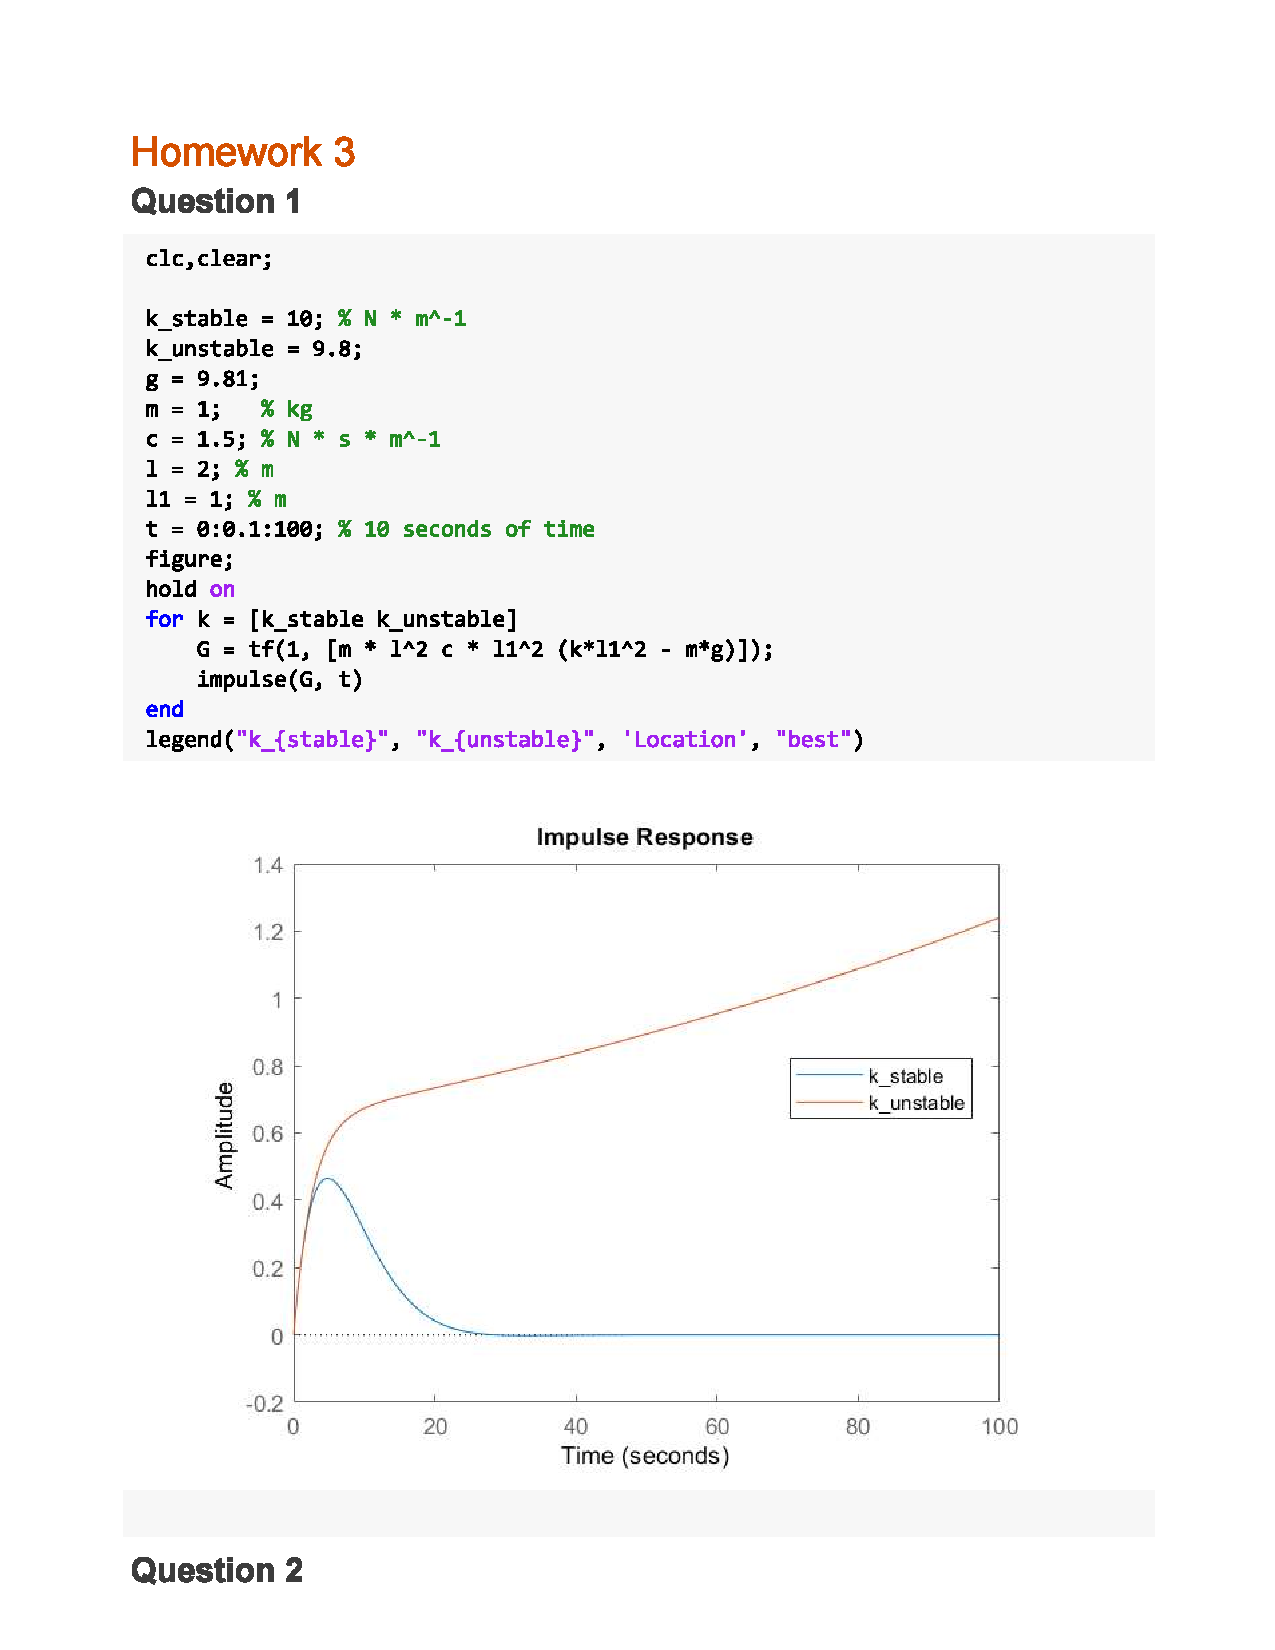
\includepdf{misc/matlab_p1.pdf}
% % Print the bibliography!
\printbibliography
\end{document}
